\section{ALGUNS CÁLCULOS CINEMÁTICOS}
Para este trabalho ser concluído, alguns cálculos cinemáticos foram necessários. Os cálculos são  as velocidades, ângulos e velocidades angulares.

Velocidades entre duas posições adjacentes num espaço 3D, são calculadas conforme a Equação \ref{v_i} \cite{Poole2011}.
\begin{equation}
	\label{v_i}
	\overrightarrow{\nu} =  \cfrac{\overrightarrow{s2} - \overrightarrow{s1}}{\tau}
\end{equation}

Os vetores $\overrightarrow{s1}$ e $\overrightarrow{s2}$ são dados espaciais em três dimensões $(X, Y, Z)$ e $\tau$ é o tempo transcorrido entre o deslocamento de um ponto ao outro. O vetor $\overrightarrow{\nu}$ possui as velocidades calculadas.

Para o cálculo de ângulos em três dimensões, primeiro os componentes devem ser transladados para uma origem comum, assim é possível usar a 
Equação \ref{angulo} como descrita em \citeonline{Edwards2006}. 
Para tal, usam-se as Equações \ref{eq1} e \ref{eq2} \cite{Poole2011}.

\begin{equation}
	\label{eq1}
	\overrightarrow{c1}^\prime =  \overrightarrow{c1} - \overrightarrow{o}
\end{equation}
\begin{equation}
	\label{eq2}
	\overrightarrow{c2}^\prime =  \overrightarrow{c2} - \overrightarrow{o}
\end{equation}

As variáveis $\overrightarrow{c1}$, $\overrightarrow{c2}$ e $\overrightarrow{o}$, são vetores representando pontos no espaço. 
O vetor $\overrightarrow{o}$ é a origem dos dois seguimentos de reta que chegam a $\overrightarrow{c1}$ e $\overrightarrow{c2}$ cada um. 
No contesto deste trabalho, $\overrightarrow{c1}$ poderia ser um ponto na coxa, $\overrightarrow{c2}$ um ponto na tíbia e $\overrightarrow{o}$ um ponto no joelho. 
Assim seria possível calcular o ângulo de um joelho, por exemplo. Veja a Figura \ref{leg}. 
As variáveis $\overrightarrow{c1}^\prime$ e $\overrightarrow{c2}^\prime$, são os vetores transladados e prontos para se calcular o ângulo de acordo com a Equação \ref{angulo} \cite{Edwards2006}.

\begin{equation}
	\label{angulo}
	\theta = \arccos{(\frac{\overrightarrow{c1}^\prime.\overrightarrow{c2}^\prime} 
	{  \left \| \overrightarrow{c1}^\prime \right \|. \left \| \overrightarrow{c2}^\prime \right \|} )} 
\end{equation}

A variável $\theta$ é um ângulo em radianos.
O operador  $\left \| \right \|$ é a distância euclidiana como definida por \citeonline{Poole2011} e seu calculo é mostrado na Equação \ref{dist_e}.

\begin{equation}
	\label{dist_e}
	  \left \| \overrightarrow{c} \right \|  =  \sqrt{\overrightarrow{c} . \overrightarrow{c}}
\end{equation}

A velocidade angular é calculada segundo a Equação \ref{vel_ang} \citeonline{Poole2011}.


\begin{equation}
	\label{vel_ang}
	\omega =  \frac{\theta_2 - \theta_1}{\tau}
\end{equation}

A variável $\omega$ é a velocidade angular em radianos por segundo, $\theta1$ e $\theta2$ são ângulos e $\tau$ o tempo transcorrido entre a medida do primeiro ângulo e do segundo.

\begin{figure}[ht]
	\centering
	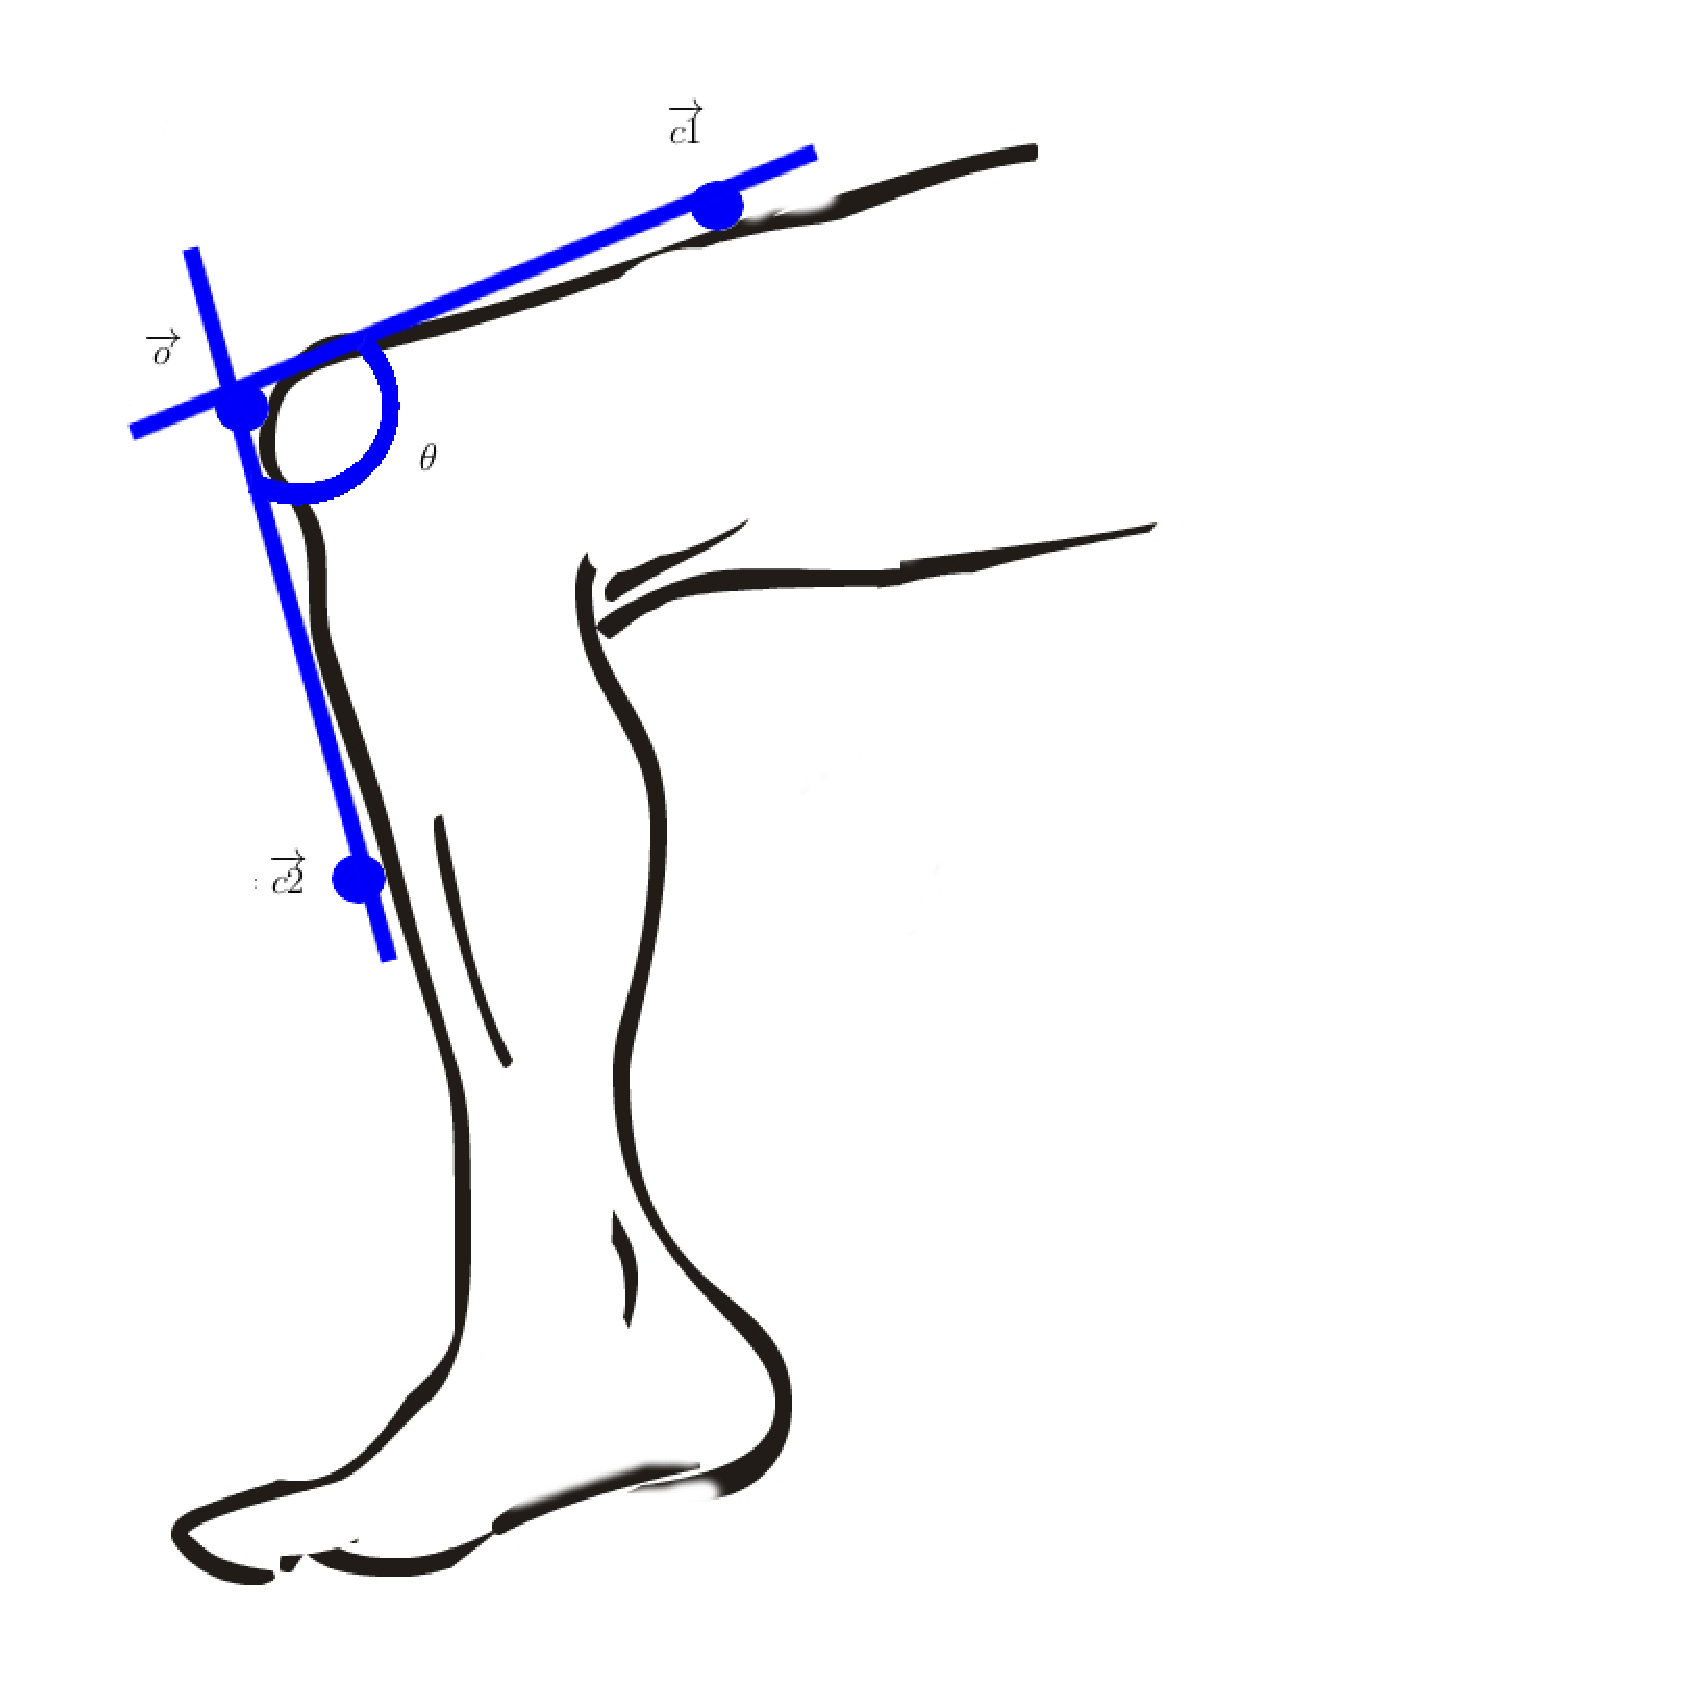
\includegraphics[width=14cm]{figuras/leg.eps}
	\caption{Exemplo hipotético de um ângulo. Adaptado de \cite{Cliparts2015}.}
	\label{leg}
\end{figure}


